\section{$\wsd$-S: A Simplification of the $\wsd$ Schedule}
\begin{figure}[t]
    \centering
        \begin{subfigure}[b]{0.3\textwidth}
            \centering
            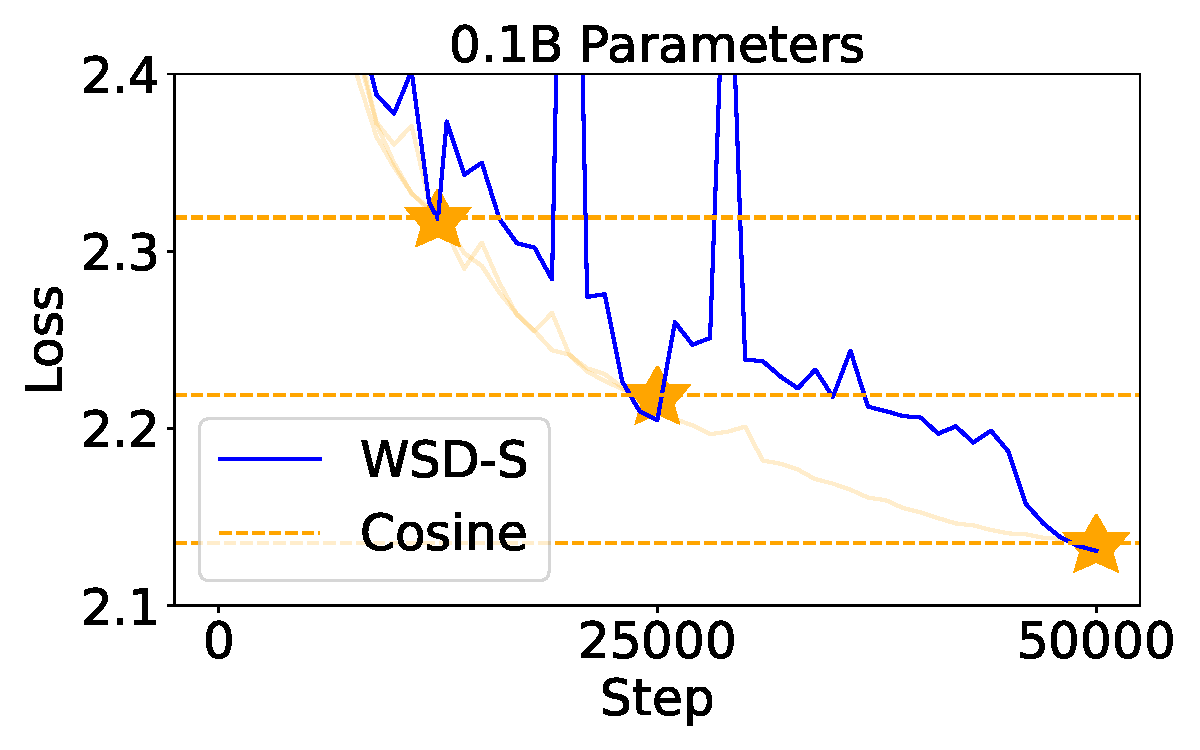
\includegraphics[width=\textwidth]{figures/arxiv/0.1B_main.pdf}
        \end{subfigure}
        \centering
        \begin{subfigure}[b]{0.3\textwidth}
            \centering
            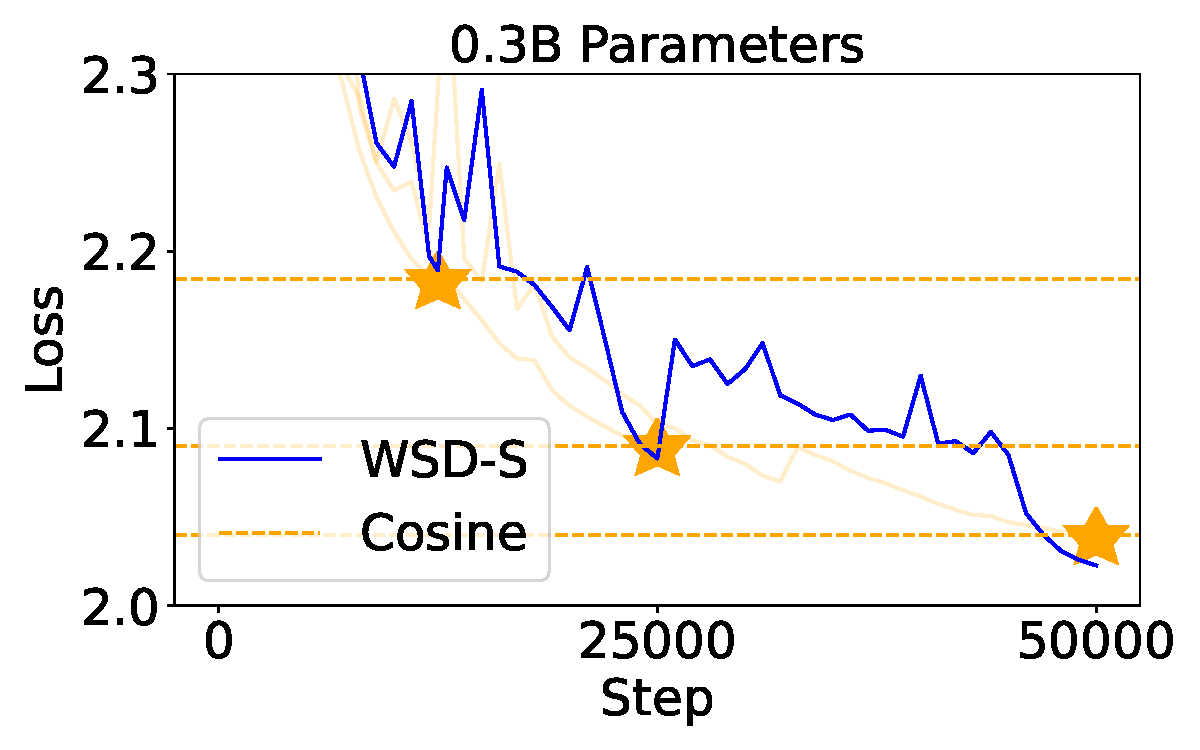
\includegraphics[width=\textwidth]{figures/arxiv/0.3B_main.pdf}
        \end{subfigure}
        \begin{subfigure}[b]{0.3\textwidth}
            \centering
            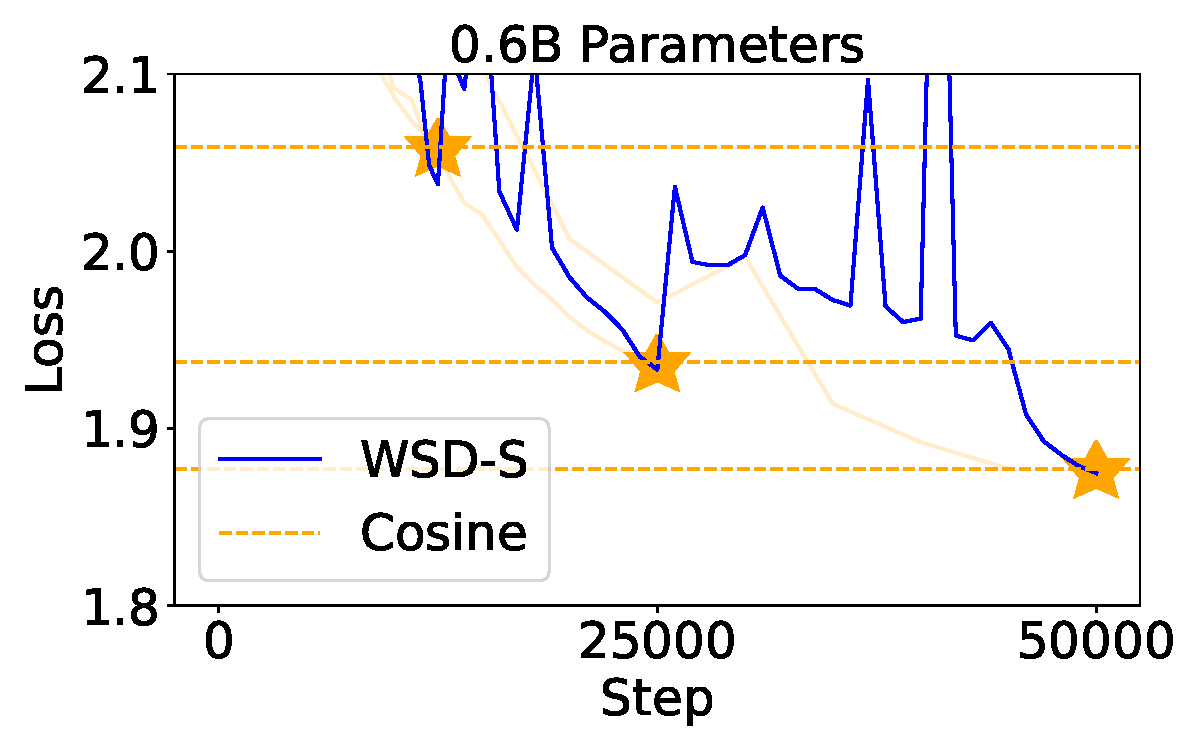
\includegraphics[width=\textwidth]{figures/arxiv/0.6B_main.pdf}
        \end{subfigure}
        \begin{subfigure}[b]{0.3\textwidth}
            \centering
            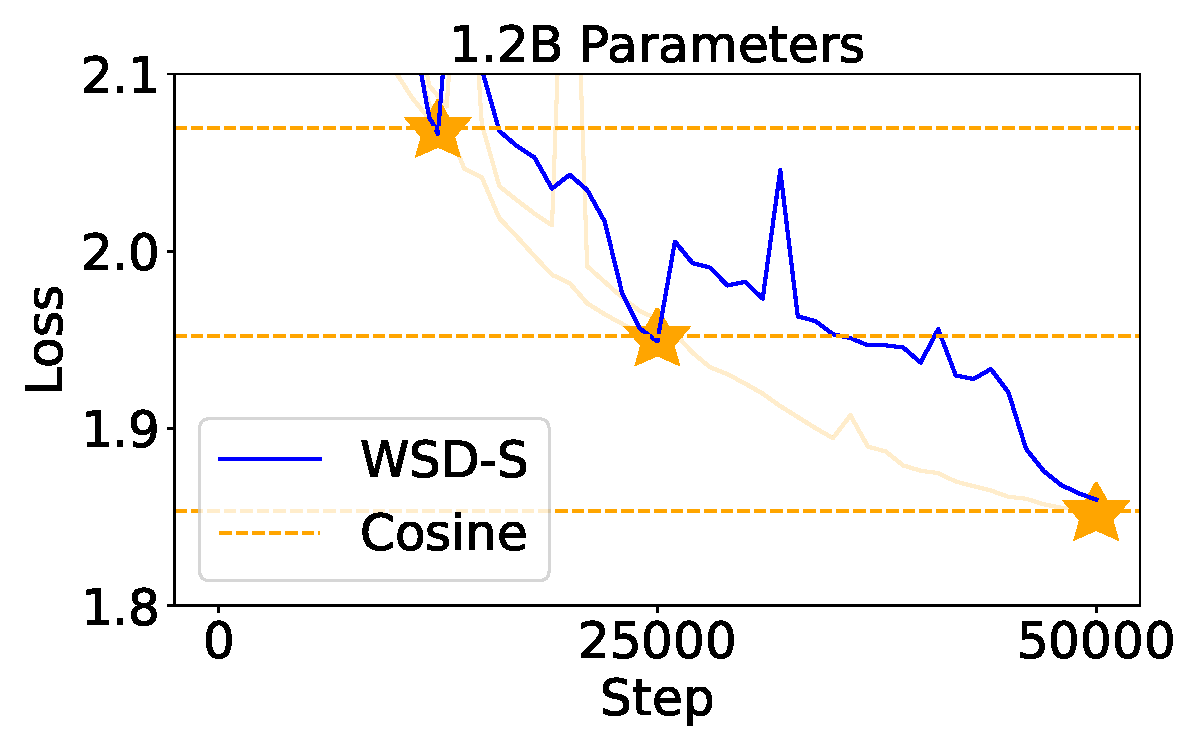
\includegraphics[width=\textwidth]{figures/arxiv/1.2B_main.pdf}
        \end{subfigure}
        \begin{subfigure}[b]{0.58\textwidth}
            \centering
            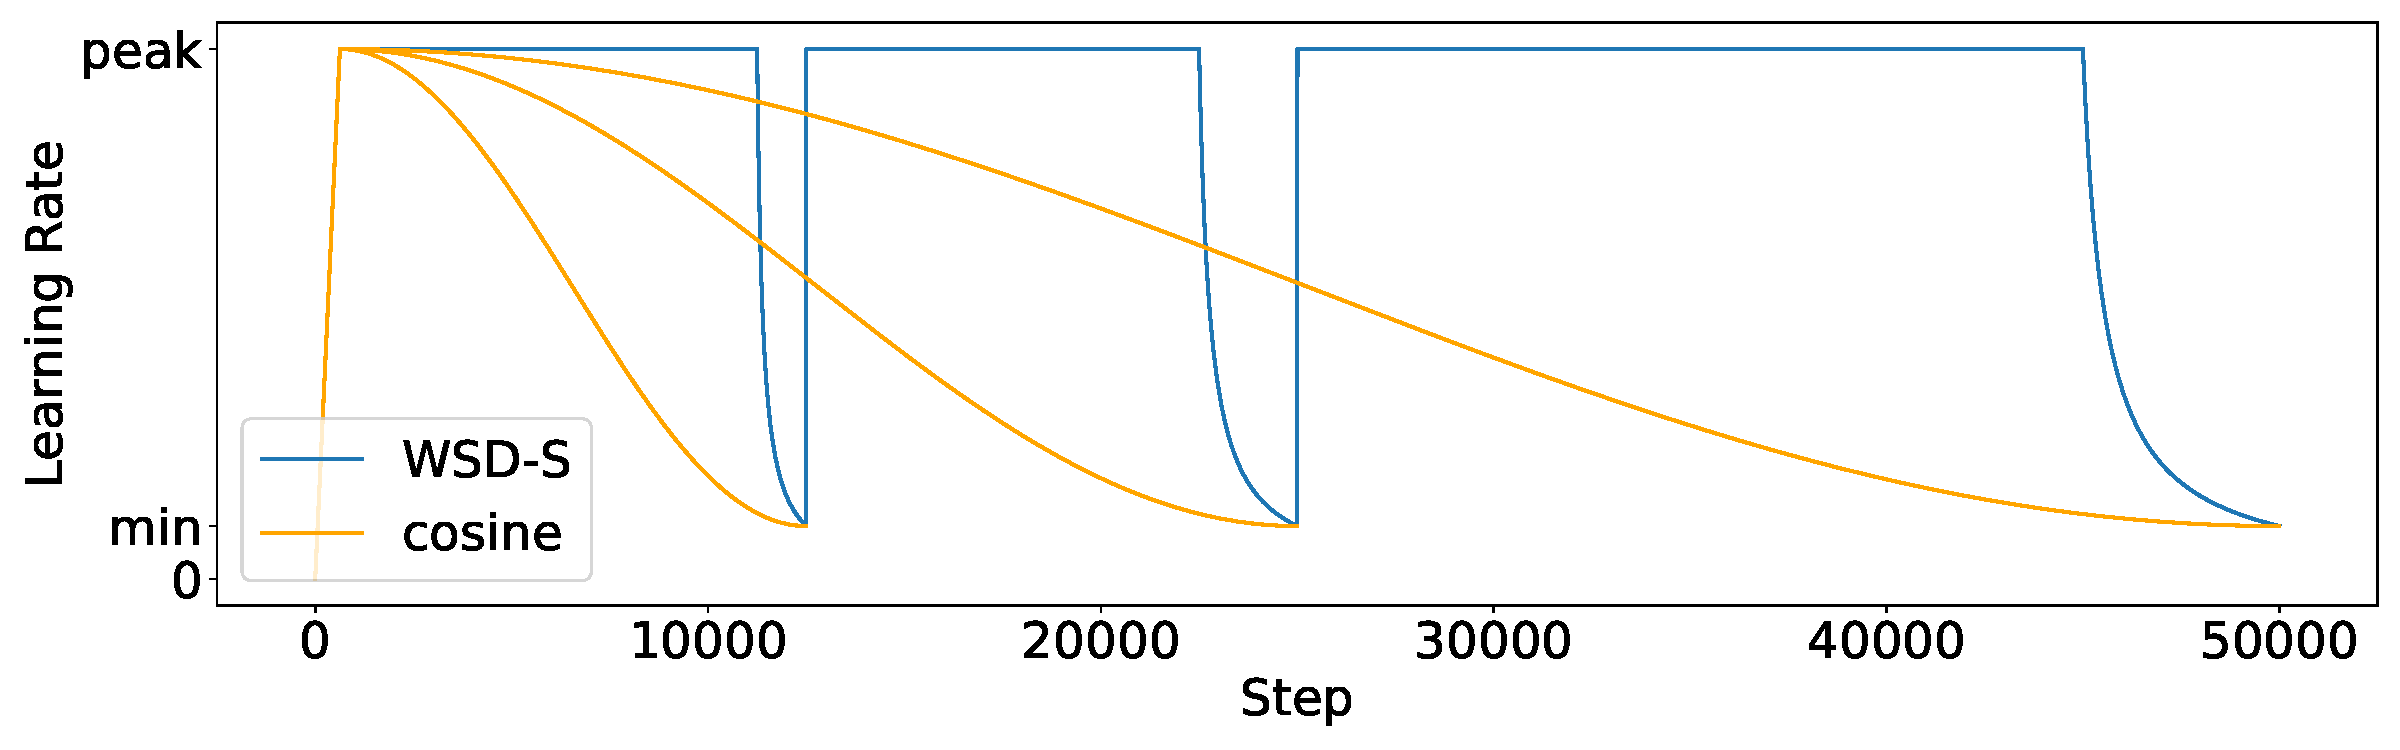
\includegraphics[width=\textwidth]{figures/arxiv/learning_rate_cosine.pdf}
        \end{subfigure}
    \caption{\textbf{Comparison with the Cosine Oracles.} We show that the $\wsds$ schedule can perform similarly to the Cosine schedules in a single run. The {\color{orange}{$\star$}} in the graphs visualize the terminating validation loss of different Cosine runs. The largest validation loss gap between the $\wsds$ and the Cosine schedules is 6e-3. The lower right figure plots the learning rate curves used in this experiment.}
    \label{fig:main}
\end{figure}


















\subsection{Method}







The goal of continual pretraining is to generate checkpoints that exhibit good performance at multiple compute budgets in one run. Formally, our goal is to achieve multiple intermediate checkpoints $\theta_{T_k}$, each corresponding to a computing budget (number of steps) $T_k$ for $k \in \{1, \ldots, K\}$.

A strong baseline to measure the performance of $\theta_{T_k}$ would be running cosine learning rates (\Cref{fig:main}, lower right) for each budget $T_k$ separately,  decays the learning rate linearly to the cosine function between $[0, \pi]$.  We will dub this \emph{oracle} method as \textbf{$\cosineoracle$}. However, $\cosineoracle$ can't be done in a single run and will incur a high total compute budgets $\sum_{k} T_k$. A simple modification to $\cosineoracle$ is to use multiple consecutive cosine learning rates between $T_{k-1}$ and $T_k$ (\Cref{fig:learningrate}, last row), which we will dub as \textbf{$\cycliccosine$}. $\cycliccosine$ only requires a total compute budgets $T_K$. However, it leads to non-negligible performance lost compared to $\cosineoracle$ (\cite{hu2024minicpm}).

Warmup-Stable-Decay (\textbf{$\wsd$}) address this issue by maintaining a {main branch} that keep using a constant learning rate after warmup process and branch off using a decaying learning rate to achieve intermediate checkpoints. One can then continue pretrain from a checkpoint in the main branch by resuming with the same constant learning rate. Formally, $\wsd$ introduce decay starting points $D_1, \ldots, D_k$ such that $T_{i - 1} < D_{i} < T_{i}$. $\wsd$ will then correspond to the following process (\Cref{fig:learningrate}, second row):
\begin{enumerate}[leftmargin=*]
    \item Get a main branch of checkpoints $\maintheta$ by running a constant learning rate schedule for $D_K$ steps.
    \item For each $k$, run a decaying learning rate schedule for $T_k - D_k$ steps starting from $\theta^{\mathrm{main}}_{D_k}$ to get $\theta_{T_k}$.
\end{enumerate}

The above process reutilizes the main branch of checkpoints $\maintheta$ for each $T_k$ and hence reduces the total compute budget to $T_K + \sum_{k} (T_k - D_k)$. 
Recall that in the river valley landscape model, the Warmup-Stable-Decay ($\wsd$) algorithm can be viewed as a combination of a large learning rate phase to speed up progress down the river and a rapid learning rate drop at the end to reduce the oscillation. Because the decay phase also makes progress along the river (see~\Cref{thm:decay-main}), we proprose a simplified version of $\wsd$, called Warmup-Stable-Decay-Simplified (\textbf{$\wsds$}), that continues with another stable phase leaving off of the end of the previous decay phase (see the first row of \Cref{{fig:learningrate}}) without separating the training process into two branches. Formally, the $\wsds$ learning rate schedule is defined as follows:
\begin{align}
\label{eq:lrs}
\eta_k = \begin{cases} 
\text{decay}(T_{i} - D_i, \maxeta, \mineta)[t - D_i] & \text{if } \exists i, D_i < t \leq T_i; \\
\maxeta & \text{otherwise.} \\
\end{cases}
\end{align}

The key difference from our methods is the choice of initialization point when retraining starts. In $\wsd$, the second stable phase uses the model before the decay phase, whereas we use the model after it.
This process is more convenient to implement because it does not require rolling back to the main branch after each decay phase. Here the learning rate decay function $\mathrm{decay}$ can take many forms that decay the learning rate from $\maxeta$ to $\mineta$ over $T_i - D_i$ steps. In this paper, we will use the inverse proportional decay function as defined in~\Cref{eq:decay} for all experiments (visualized in~\Cref{fig:learningrate}, first two rows).

\begin{align}
\label{eq:decay}
\frac{1}{\text{decay}(T, \mineta, \maxeta)} &= \left[ \frac{t}{T} \frac{1}{\mineta} + \left(1 - \frac{t}{T}\right) \frac{1}{\maxeta} \ \Bigg| \ t \in \{0, 1, \ldots, T\} \right]. 
\end{align}

This function is motivated by the analysis on quadratic functions in~\Cref{thm:decay-main}. The reciprocal
 of the learning rate linearly interpolates from the reciprocal
 of maximal to the reciprocal
 of minimal learning rate.
